\documentclass{article}
\usepackage[utf8]{inputenc}
\usepackage[english, russian]{babel}
\usepackage{graphicx}
\graphicspath{ {./graphics/} }
\usepackage[a4paper, total={6in, 8in}]{geometry}
\pagestyle{empty} %
\usepackage[pageanchor]{hyperref}
\usepackage{enumitem}
\usepackage{listings}
\usepackage{amssymb}
\usepackage{amsmath}
\usepackage{indentfirst}
\usepackage{tikz}

\newcommand{\kaucher}{
  \begin{tikzpicture}
    \draw (0, 0) circle (0.6ex);
    \draw (-0.6ex, 0) -- (0.6ex, 0);
  \end{tikzpicture}%
}

\begin{document}
  \begin{titlepage}
    \begin{center}
      Санкт-Петербургский политехнический университет \\Петра Великого
    \end{center}

    \begin{center}
      Физико-механический институт
    \end{center}

    \begin{center}
      Высшая школа прикладной математики и вычислительной\\ физики
    \end{center}

    \vspace{8em}

    \begin{center}
      \textbf{Отчет по лабораторной работе №2}\\
      \textbf{“Интервальный анализ”}
    \end{center}

    \vspace{\fill}

    \begin{flushright}
      \noindentВыполнили студент группы 5030102/10201:
      \hfill
      Скворцов Владимир Сергеевич \\
    \end{flushright}
    Преподаватель: \hfill Баженов Александр Николаевич

    \vspace{12em}

    \begin{center}
      Санкт-Петербург\\
      2024
    \end{center}
  \end{titlepage}

  \tableofcontents

  \newpage

  \section{Постановка задачи}

  Дан набор ИСЛАУ \ref{eq:islae}

  \begin{equation} \label{eq:islae}
    \mathbf{A}x = \mathbf{b}, \ x = (x_1, x_2)
  \end{equation}

  с матрицей и вектором правой части:

  \begin{equation} \label{eq:problem_1}
    \mathbf{A} = \begin{pmatrix}
      [0.65, 1.25] & [0.7, 1.3] \\
      [0.75, 1.35] & [0.7, 1.3]
    \end{pmatrix},
    ~
    \mathbf{b} = \begin{pmatrix}
      [2.75, 3.15] \\
      [2.85, 3.25]
    \end{pmatrix};
  \end{equation}

  \begin{equation} \label{eq:problem_2}
    \mathbf{A} = \begin{pmatrix}
      [0.65, 1.25] & [0.7, 1.3] \\
      [0.75, 1.35] & [0.7, 1.3] \\
      [0.8, 1.4] & [0.7, 1.3]
    \end{pmatrix},
    ~
    \mathbf{b} = \begin{pmatrix}
      [2.75, 3.15] \\
      [2.85, 3.25] \\
      [2.90, 3.3]
    \end{pmatrix};
  \end{equation}

  \begin{equation} \label{eq:problem_3}
    \mathbf{A} = \begin{pmatrix}
      [0.65, 1.25] & [0.7, 1.3] \\
      [0.75, 1.35] & [0.7, 1.3] \\
      [0.8, 1.4] & [0.7, 1.3] \\
      [-0.3, 0.3] & [0.7, 1.3]
    \end{pmatrix},
    ~
    \mathbf{b} = \begin{pmatrix}
      [2.75, 3.15] \\
      [2.85, 3.25] \\
      [2.90, 3.3] \\
      [1.8, 2.2]
    \end{pmatrix}.
  \end{equation}

  Необходимо:

  \begin{itemize}
    \item Проверить непустоту допускового множества ИСЛАУ \ref{eq:islae},
    \item Построить график функционала \( \text{Tol}(x) \) для \ref{eq:islae},
    \item Построить допусковое множество ИСЛАУ \ref{eq:islae},
    \item Найти \( \text{argmax} \ \text{Tol} \) и образующие допускового
      функционала.
  \end{itemize}

  Для достижения непустого допускового множества провести коррекцию ИСЛАУ
  \ref{eq:islae}:

  \begin{itemize}
    \item Правой части ИСЛАУ --- \( b \)-коррекция,
    \item Матрицы ИСЛАУ --- \( A \)-коррекция,
    \item Комбинацией предыдущих методов с одновременным изменением
      правой части и матрицы ИСЛАУ — \( Ab \)-коррекция.
  \end{itemize}

  Для всех видов коррекции построить график функционала
  \( \text{Tol} (x) \), допускового множества, отобразить
  \( \text{argmax} \ \text{Tol} \) и найденные ранее частные решения набора
  СЛАУ.

  \section{Необходимая теория}

  \subsection{Допусковое множество}

  Пусть даны интервальная \( m \times n \) матрица \( \mathbf{A} \) и
  интервальный аетор правой части \( \mathbf{b} \).

  \vspace{\baselineskip}

  \emph{Допусковым множеством} решений ИСЛАУ называется множетсво

  \begin{equation} \label{eq:tol_set_of_solutions}
    \Xi_{\text{tol}} (\mathbf{A}, \mathbf{b}) \stackrel{\text{def}}{=}
      \left \{ x \in \mathbb{R}^n \mid \forall A \in \mathbf{A} \ \exists b \in \mathbf{b}: \ Ax = b \right \}.
  \end{equation}

  \vspace{\baselineskip}

  Функционалом \( \text{Tol} (x): \mathbb{R}^n \times \mathbb{IR}^{m \times n} \times \mathbb{IR}^m \to \mathbb{R} \)
  называется выражение

  \begin{equation} \label{eq:tol}
    \text{Tol} (x, \mathbf{A}, \mathbf{b}) \stackrel{\text{def}}{=}
      \min_{1 \leq i \leq m} \left \{ \text{rad} \mathbf{b}_i - \left | \text{mid} \mathbf{b}_i - \sum_{j=1}^n \mathbf{a}_{ij} x_j \right | \right \}.
  \end{equation}

  Тогда принадлежность \( x \in \Xi_{\text{tol}} (\mathbf{A}, \mathbf{b}) \)
  равносильна \( \text{Tol} (x, \mathbf{A}, \mathbf{b}) \geq 0 \), то есть
  допусковое множество решений интервальной линейной системы
  \( \mathbf{A} x = \mathbf{b} \) есть множество уровня
  \[
    \left \{ x \in \mathbb{R}^n \mid \text{Tol} (x, \mathbf{A}, \mathbf{b}) \geq 0 \right \}
  \]
  функционала \( \text{Tol} \).

  \vspace{\baselineskip}

  \subsection{\( b \)-коррекция ИСЛАУ}

  Пусть матрица \( \mathbf{A} \) ИСЛАУ неизменна, и значения
  \( \text{mid} \mathbf{b}_i, i \in \overline{1,m} \) зафиксированы. Тогда
  расширение вектора \( \mathbf{b} \) путем его замены на вектор

  \begin{equation} \label{eq:b-correction}
    \mathbf{b} + K\mathbf{e}, \ K \ge 0, \ \mathbf{e} = ([-1, 1], \dots, [-1, 1])^T
  \end{equation}

  приведет к тому, что значение абсолютного максимума \( T \) распознаю-
  щего функционала \( \text{Tol} (x, \mathbf{A}, \mathbf{b}) \) возрастет на
  постоянную \( K \):
  \[
    \max_{x \in \mathbb{R}^n} \text{Tol} (x, \mathbf{A}, \mathbf{b} + K \mathbf{e})
      = \max_{x \in \mathbb{R}^n} \text{Tol} (x, \mathbf{A}, \mathbf{b}) + K = T + K
  \]
  прием \( \text{argmax} \ \text{Tol} \) — положение точки \( T \) ---
  не изменится.

  \subsection{\( A \)-коррекция ИСЛАУ}

  \( A \)-коррекцией ИСЛАУ \( \mathbf{A}x = \mathbf{b} \) заключается
  в замене матрицы \( \mathbf{A} \) ее интервальной матрицей
  \( \mathbf{A} \kaucher \mathbf{E} \) такой, что
  \[
    \text{rad} (\mathbf{A} \kaucher \mathbf{E}) < \text{rad} \mathbf{A}, \
    \text{mid} (\mathbf{A} \kaucher \mathbf{E}) = \text{mid} \mathbf{A}, \
    \mathbf{e}_{ij} = [-e_{ij}, e_{ij}].
  \]

  \subsection{\( Ab \)-коррекция ИСЛАУ}

  \( Ab \)-коррекцией ИСЛАУ \( \mathbf{A}x = \mathbf{b} \) заключается
  в комбинированном применении \( A \)-коррекци и \( b \)-коррекции,
  при этом первый этап процесса --- сужение элементов матрицы А,
  второй этап --- уширение вектора правой части \( b \).

  \section{Реализаця}

  Лабораторная работа выполнена на языке программирования Python. В ходе
  работы были также использованы библиотеки \verb!numpy! и
  \verb!matplotlib!.

  Ссылка на GitHub репозиторий:
  \href{https://github.com/vladimir-skvortsov/spbstu-interval-anylysis}{https://github.com/vladimir-skvortsov/spbstu-interval-anylysis}

  % \subsection{Алгоритм проверки непустоты допускового множества ИСЛАУ}

  % Пусть дана интервальная система линейных алгебраических уравнений
  % (ИСЛАУ) \( \mathbf{A}x = \mathbf{b} \), где \( \mathbf{A} \) ---
  % интервальная матрица, а \( \mathbf{b} \) — интервальный вектор.
  % Необходимо определить, является ли допусковое множество решений
  % \( \Xi_{\text{tol}}(\mathbf{A}, \mathbf{b}) \) непустым. Для этого
  % используется следующий алгоритм:

  % \textbf{Начальные параметры}:
  % \begin{itemize}
  %   \item \( \varepsilon > 0 \) --- заданная точность для определения
  %     максимума функции толерантности.
  %   \item \( x_0 \) --- начальное приближение, составляется из средних
  %     значений интервалов \( \text{mid} \mathbf{A} \) и
  %     \( \text{mid} \mathbf{b} \).
  % \end{itemize}

  % \textbf{Алгоритм}:
  % \begin{enumerate}
  %   \item Вычисляем начальное приближение \( x_0 \) путём решения системы
  %     \( \text{mid}(\mathbf{A}) \mathbf{x} = \text{mid}(\mathbf{b}) \),
  %   \item Используем метод оптимизации (например, квазиньютоновские
  %     методы) для нахождения минимума функции
  %     \( -\text{Tol}(\mathbf{x}, \mathbf{A}, \mathbf{b}) \), начиная с точки
  %     \( \mathbf{x}_0 \) с точностью \( \varepsilon \).
  %   \item Если изменение значения функции между итерациями становится
  %     меньше \( \varepsilon \), останавливаем поиск максимума.
  %   \item Если найденное максимальное значение
  %     \( \text{Tol}(\mathbf{x}^*, \mathbf{A}, \mathbf{b}) \geqslant 0 \), где
  %     \( x^* \) --- найденная точка максимума, то допусковое множество
  %     \( \Xi_{\text{tol}}(\mathbf{A}, \mathbf{b}) \) непусто. В противном
  %     случае, пусто.
  % \end{enumerate}

  \clearpage

  \section{Результаты}

  \subsection{Максимум распознающего функционала}

  Максимум со значением \( T = -0.7 \) расположен в точке
  \( \tau = (1, 2)^T \), для всех формулировок. Образующая функционала в
  начальном случае для \ref{eq:problem_3}:

  \begin{equation}
    \mathbf{v} = \begin{pmatrix}
      -0.7 \\
      -0.7 \\
      -0.7 \\
      -0.7
    \end{pmatrix}
  \end{equation}

  В таком случае допусковое множество пусто.

  \begin{figure}[htbp!]
		\begin{center}
			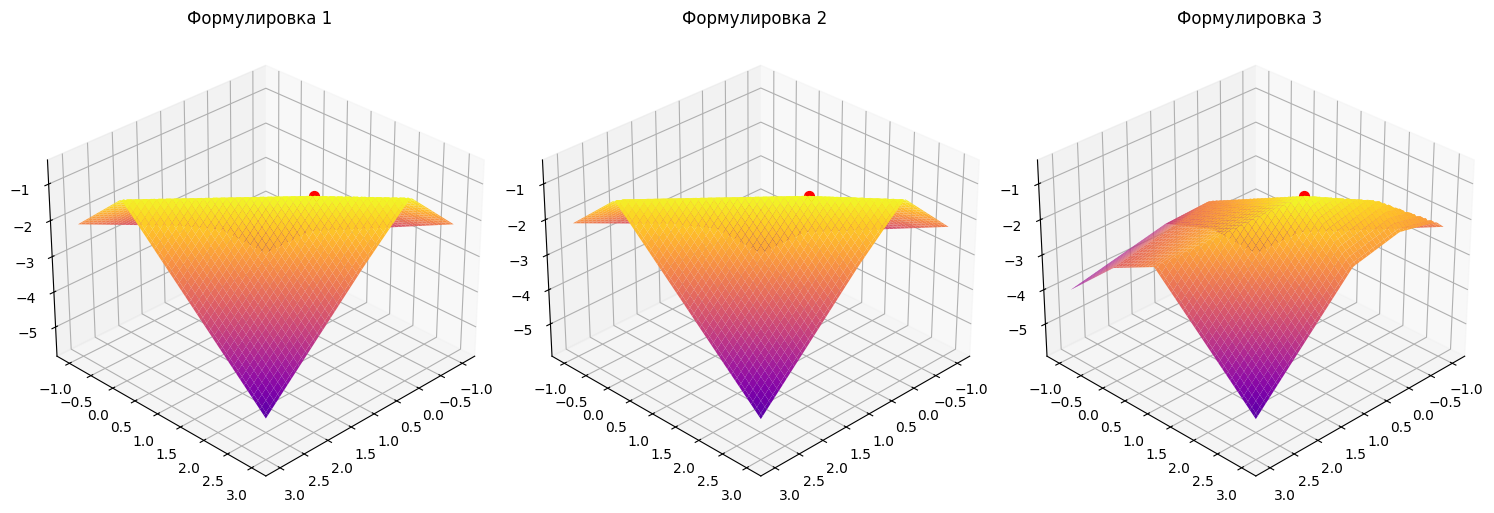
\includegraphics[width = \textwidth]{tol}
			\caption{Расположение максимума распознающего функционала}
      \label{figure:tol}
		\end{center}
	\end{figure}

  \subsection{Достижение разрешимости за счёт коррекции левой части
  (А-коррекция)}

  Для нахождения интервала допустимых значений \( e \) для
  \( A \)-коррекции формулировки \ref{eq:problem_1} выполним следующие
  действия:

  \begin{equation*}
    T = \text{Tol}(\tau, \mathbf{A}, \mathbf{b}) = -0.7 \Rightarrow |T| = 0.7,
  \end{equation*}
  \begin{equation*}
    \tau = \text{Arg} \max_{x \in \mathbb{R}^n}
    \text{Tol}(x, \mathbf{A}, \mathbf{b}) = (1, 2)^T \Rightarrow
    |\tau_1| = 1, \ |\tau_2| = 2.
  \end{equation*}

  Найдем точечную матрицу

  \begin{equation*}
    \text{rad} A = \begin{pmatrix}
      0.3 & 0.3 \\
      0.3 & 0.3 \\
      0.3 & 0.3 \\
      0.3 & 0.3
    \end{pmatrix}.
  \end{equation*}

  и решим следующую систему неравенств:

  \begin{equation*}
    \begin{cases}
      0 \leqslant e \leqslant 0.3, \\
      e + 2e = K \geqslant |T| = 0.7
    \end{cases} \Rightarrow 0.2(3) \leqslant e \leqslant 0.3.
  \end{equation*}

  Остановим свой выбор на
  \( e_{\text{mid}} = \frac{0.2(3) + 0.3}{2} = 0.2(6) \). Тогда ИСЛАУ
  \( \mathbf{A}x = \mathbf{b} \) преобретает соедующий вид:

  \begin{equation*}
    \mathbf{A} = \begin{pmatrix}
      [0.917, 0.983] & [0.967, 1.033] \\
      [1.017, 1.083] & [0.967, 1.033] \\
      [1.067, 1.133] & [0.967, 1.033] \\
      [-0.033, 0.033] & [0.967, 1.033] \\
    \end{pmatrix}, \
    \mathbf{b} = \begin{pmatrix}
      [2.75, 3.15] \\
      [2.85, 3.25] \\
      [2.90, 3.3] \\
      [1.8, 2.2]
    \end{pmatrix}.
  \end{equation*}

  Максимум со значением \( T = 0.1 \) расположен в точке
  \( \tau = (1, 2)^T \).

  \begin{figure}[htbp!]
		\begin{center}
			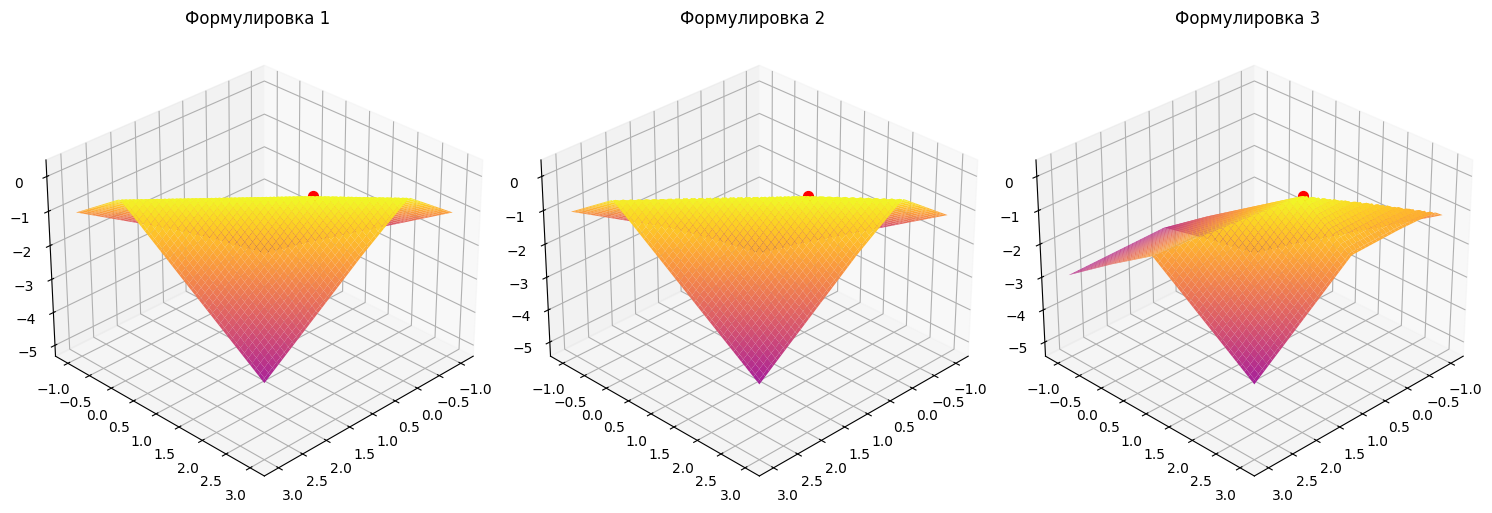
\includegraphics[width = \textwidth]{tol_a_corrected}
			\caption{Поверхности распознающих функционалов после
        \( A \)-корректировки}
      \label{figure:tol_a_corrected}
		\end{center}
	\end{figure}

  \begin{figure}[htbp!]
		\begin{center}
			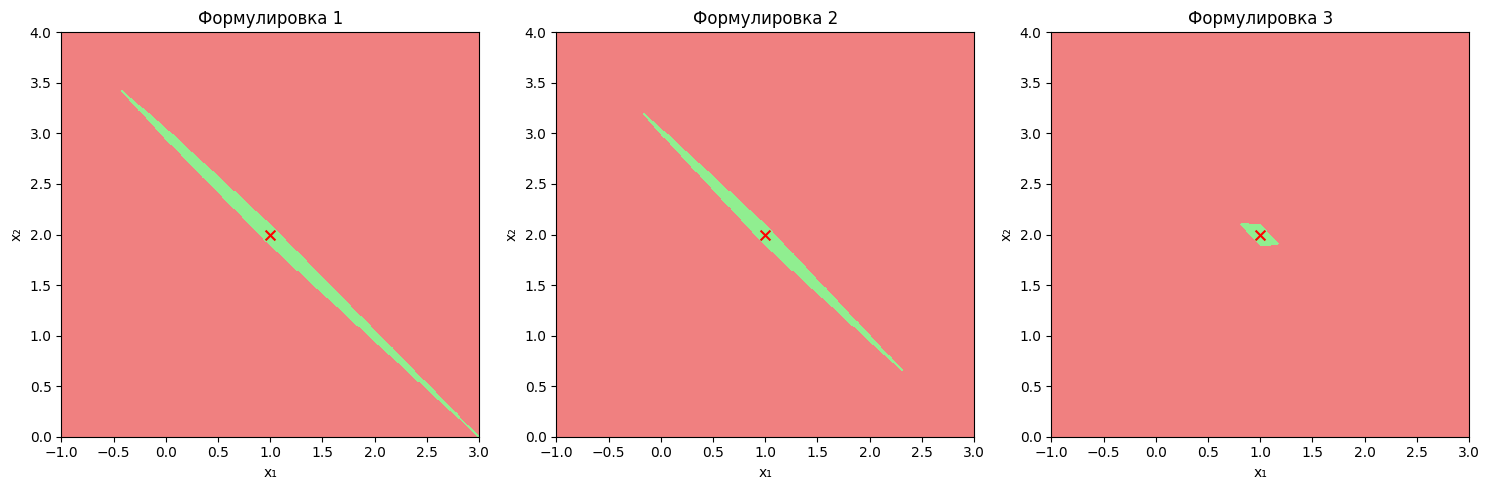
\includegraphics[width = \textwidth]{tol_functional_a_corrected}
			\caption{Допусковое множество решений после \( A \)-корректировки}
      \label{figure:tol_functional_a_corrected}
		\end{center}
	\end{figure}

  \subsection{Достижение разрешимости за счёт коррекции правой части
  (b-коррекция)}

  Для построения интервальной матрицы был взят коэффициент \( K = 1 \) для
  всех ИСЛАУ. Для примера, задача \ref{eq:problem_3}, принимает вид:

  \begin{equation*}
    \mathbf{A} = \begin{pmatrix}
      [0.65, 1.25] & [0.7, 1.3] \\
      [0.75, 1.35] & [0.7, 1.3] \\
      [0.8, 1.4] & [0.7, 1.3] \\
      [-0.3, 0.3] & [0.7, 1.3]
    \end{pmatrix},
    ~
    \mathbf{b} = \begin{pmatrix}
      [1.75, 4.15] \\
      [1.85, 4.25] \\
      [1.9, 4.3] \\
      [0.8, 3.2]
    \end{pmatrix}.
  \end{equation*}

  \begin{figure}[htbp!]
		\begin{center}
			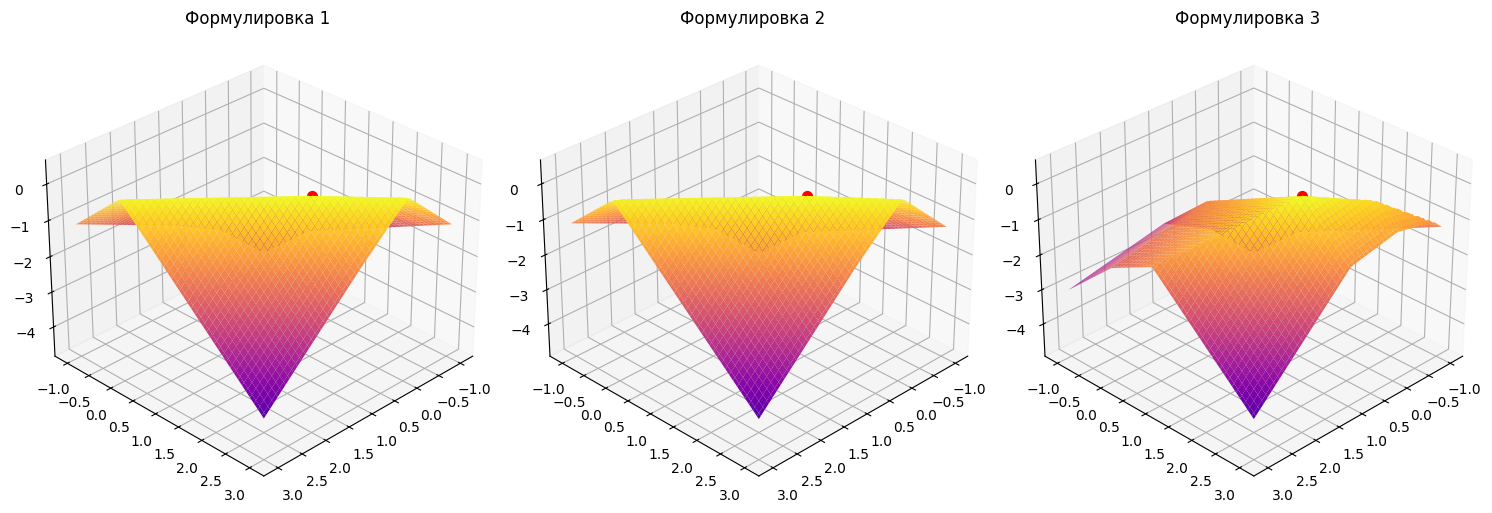
\includegraphics[width = \textwidth]{tol_b_corrected}
			\caption{Поверхности распознающих функционалов после
        \( b \)-корректировки}
      \label{figure:tol_b_corrected}
		\end{center}
	\end{figure}

  \begin{figure}[htbp!]
		\begin{center}
			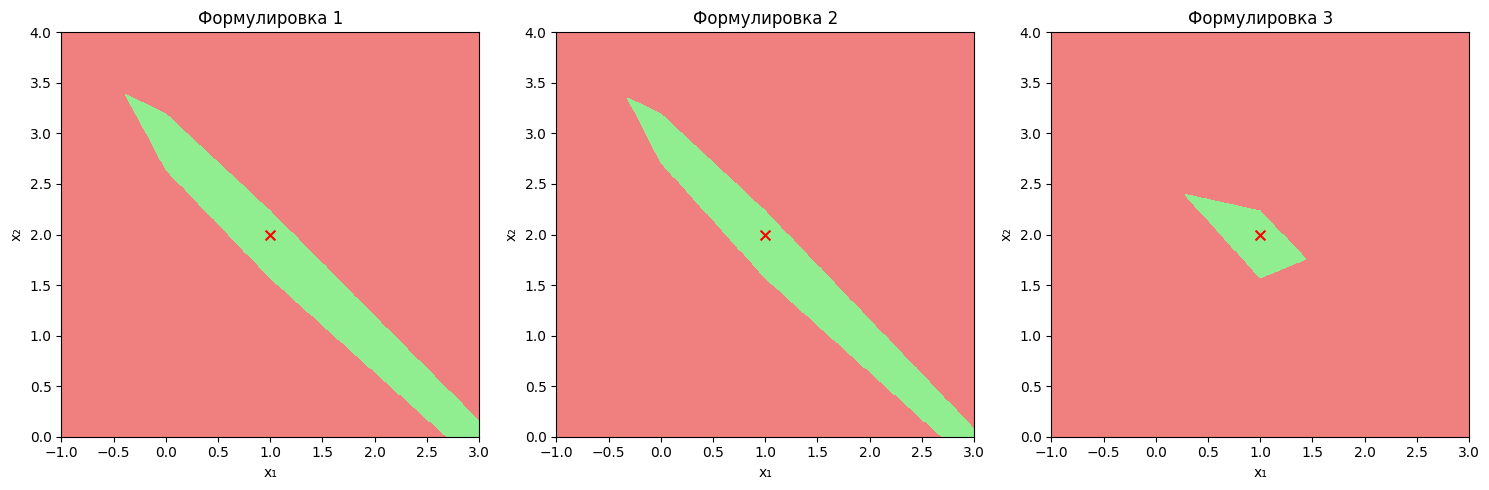
\includegraphics[width = \textwidth]{tol_functional_b_corrected}
			\caption{Допусковое множество решений после \( b \)-корректировки}
      \label{figure:tol_functional_b_corrected}
		\end{center}
	\end{figure}

  Минимальное значение \( K = 0.7 \) в предельном переходе неотрицательной
  области сводится к точке \( \tau = (1, 2)^T \).

  \subsection{Достижение разрешимости за счёт Ab-коррекции}

  Сначала проводилось сужение левой части (\( A \)-коррекция), затем
  расширение правой части (\( b \)-коррекция) с коэффициентом \( K = 1 \).

  \begin{figure}[htbp!]
		\begin{center}
			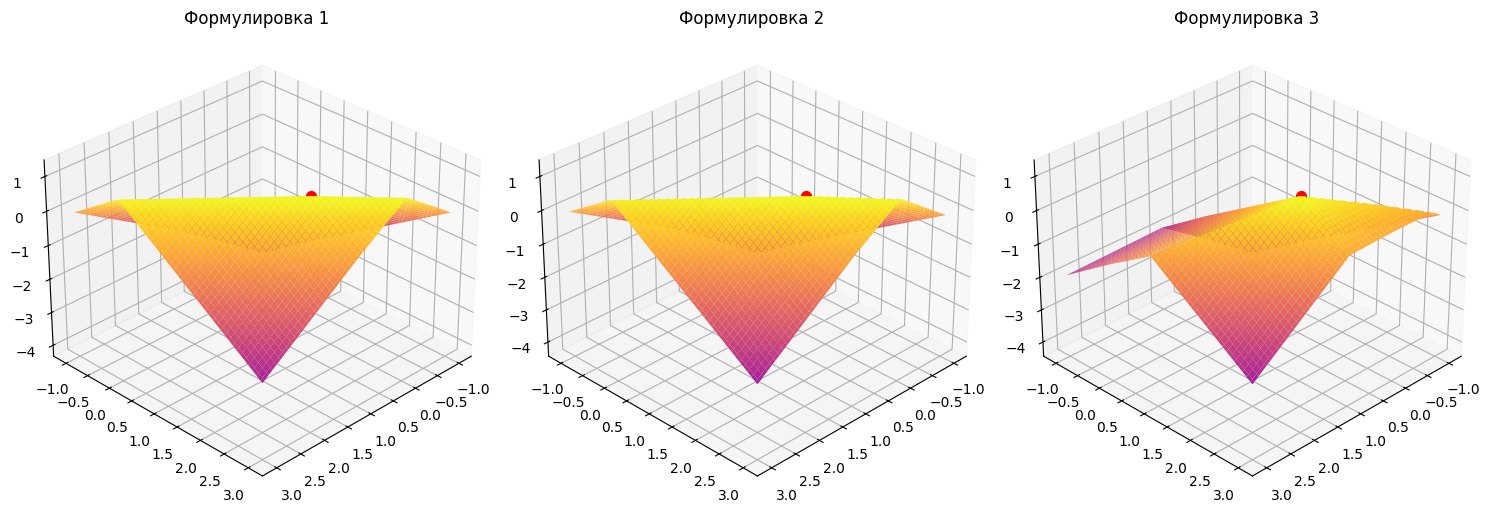
\includegraphics[width = \textwidth]{tol_ab_corrected}
			\caption{Поверхности распознающих функционалов после
        \( Ab \)-корректировки}
      \label{figure:tol_ab_corrected}
		\end{center}
	\end{figure}

  \begin{figure}[htbp!]
		\begin{center}
			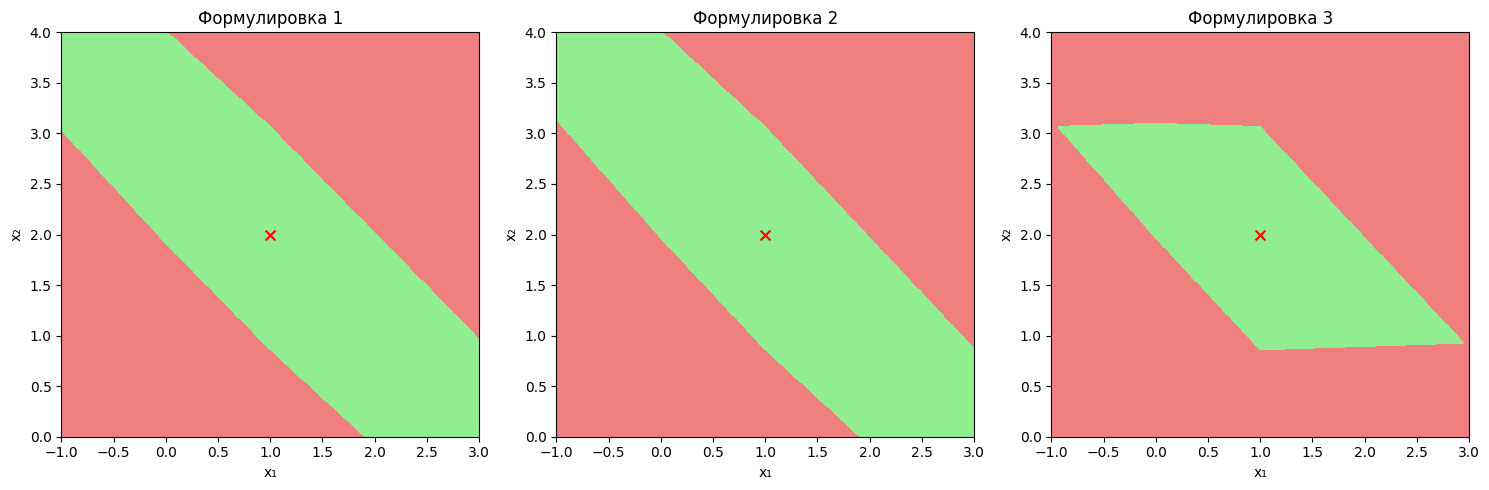
\includegraphics[width = \textwidth]{tol_functional_ab_corrected}
			\caption{Допусковое множество решений после \( Ab \)-корректировки}
      \label{figure:tol_functional_ab_corrected}
		\end{center}
	\end{figure}

  \section{Выводы}

  \begin{itemize}
    \item В результате работы установлено, что для заданных ИСЛАУ
    допусковое множество решений является пустым, поскольку максимальное
    значение распознающего функционала \( T = -0.7 \) оказалось меньше
    нуля. Это свидетельствует о несовместимости исходной системы в
    заданных интервалах.
    \item Для достижения разрешимости системы были применены методы
    коррекции правой части (\( b \)-коррекция) и матрицы коэффициентов
    (\( A \)-коррекция). В частности, после применения \( b \)-коррекции с
    коэффициентом \( K = 1 \) удалось получить положительное значение
    распознающего функционала \( T = 0.3 \). Это указывает на то, что
    скорректированная система обладает непустым допусковым множеством
    решений.
    \item Применение \( A \)-коррекции также обеспечило разрешимость ИСЛАУ.
    Скорректированная матрица коэффициентов позволила добиться
    положительного значения распознающего функционала и определить
    допусковое множество решений, что подтверждает эффективность данного
    метода.
    \item Анализ графиков допусковых множеств и распознающего функционала
    показал,что после коррекции форма поверхности \( \text{Tol} (x) \)
    изменилась.Это отражает влияние коррекции на свойства системы. Кроме
    того, смещение максимума распознающего функционала подтверждает
    улучшение совместимости системы.
  \end{itemize}


\end{document}
